\chapter{Implementation \& Experiments} \label{experiments}

In this chapter, we will discuss the implementation of our proposed algorithm in practice. Recall that we aim to solve the challenges of ``computational cost'' and ``adaptability'' \cite{lima_quest_2023} to the ``15-Minute City" problem with an algorithmic approach, it is important that the algorithm is implemented in a low-level language to promote efficiency in our experiments.

\section{Implementation}

Rust is a low-level programming language which has gained significant popularity in the field of Computer Science in recent years. It is a statically typed language to promote safety and concurrency. Rust achieves these goals by using a unique ownership model to manage memory allocation and deallocation at compile time, preventing common errors such as null pointer dereferencing and data races. This makes Rust an attractive choice for programming where performance and reliability are critical.

In our implementation of the algorithm, we opted to build the algorithm with the minimum amount of non-official crates (packages for Rust). With this in mind, we have used the \verb|petgraph| and the \verb|ordered_float| crates: \verb|petgraph| \cite{petgraph} supports an undirected graph data structure \verb|UnGraphMap| while \verb|ordered_float::NotNan| \cite{ordered_float} is a necessary extension to the priority queue as the standard library's Binary Heap implementation only supports Integer ordering as according to \verb|754-2008 - IEEE Standard for Floating-Point Arithmetic| \cite{IEEE}. It is important to note that while Fibonacci Heap has been used in our solution, we have opted to use a built in Binary Heap in our code, it is due to the fact that there is a lack of available implementation of Fibonacci Heaps in Rust.

The implementation of our code takes 2 \verb|csv| files in inputs, \verb|nodes.csv| and \verb|edges.csv|. \verb|nodes.csv| contains the nodes identifier in the graph, along with a \verb|label| field for the type of the service the node contains, or it can be empty. \verb|edges.csv| contains the \verb|source|, \verb|target| and \verb|weight| for every edge in our graph. Precisely, the node identifier fields \verb|id|, \verb|source|, and \verb|target| should be represented by integers, which is \verb|u64| in Rust, where \verb|u| stands for ``unsigned''. Furthermore, \verb|label| should be a string or empty, and \verb|weight| should be of type float, or \verb|f64|. The table \ref{tab:data_type} shows a summary of the data types for each input variable.

\begin{table}[htbp]
    \begin{center}
        \caption{Summary of input data type}
        \label{tab:data_type}
        \begin{tabular}{ ccc }
            \hline
            \textbf{Input} & \textbf{Data Type} & \textbf{Rust Type} \\
            \hline
            \hline
            \verb|id| & Integer & \verb|u64| \\
            \hline
            \verb|source| & Integer & \verb|u64| \\
            \hline
            \verb|target| & Integer & \verb|u64| \\
            \hline
            \verb|weight| & Float & \verb|f64| \\
            \hline
            \verb|label| & String & \verb|String| \\
            \hline
        \end{tabular}
    \end{center}
\end{table}

The algorithm is implemented in Rust as a single thread application. In practice, it would be vise to parallelise the algorithm to take advantage of the concurrency ability of Rust to utilise the multi-core processors in modern computers.

\section{Data Preparation} \label{data_preparation}

The data preparation for the algorithm is done in Python, this is due to the flexible and well-supported nature of the programming language. In this experiment, we obtain the map data from OpenStreetMap via the OpenStreetMap API and the \verb|osmnx| library \cite{OSMnx}. As oppose to Google Maps, OpenStreetMap does not require an API key in order to download map data. The obtained map data is stored as a \verb|MultiDiGraph| object from the \verb|NetworkX| library \cite{SciPyProceedings_11}, the \verb|MultiDiGraph| object supports a directed graph and allows for multiple edges between any two nodes, this will be converted to a \verb|MultiGraph| object which represents an undirected graph and duplicated edges will be removed in the subsequent steps detailed below.

The list below lays out the steps taken to obtain the map data in high-level:

\begin{enumerate}
    \item Download map data as an \verb|MultiDiGraph| object with the \verb|osmnx| library and the \verb|network_type| set as \verb|all|. Area could be selected by one of the following:
    \begin{itemize}
        \item City administration boundary
        \item A bounding box of coordinates
        \item A user-defined radius from a location given by its coordinates
    \end{itemize}
    \item The graph is simplified by merging nodes that are within 10 metres of each other, this eliminates having too many nodes at junctions and pedestrian areas.
    \item The directed graph is transformed into an undirected graph.
    \item For the selected service locations
    \begin{itemize}
        \item Locate the closest point of the closest edge (i.e. street) from each location.
        \item For each location, insert a new node to the graph and replace the original edge by 2 newly inserted edges to connect the new node.
    \end{itemize}
    \item Remove parallel edges by only retaining the edge with the minimum weight.
    \item Export the graph data into \verb|nodes.csv| and \verb|edges.csv|.
\end{enumerate}

\textbf{Show visualisation of how nodes are inserted}

\section{Experiment} \label{padua}

The experiments in this thesis are conducted on a MacBook Pro with a M1 Pro SoC, which is an ARM-based processor. The machine has 8 CPU cores and 16GB of RAM. The operating system is macOS Sonoma 14.5. The Rust compiler version is 1.78.0. The Python version is 3.12.0. The versions of the Python libraries and Rust crates used are as follows:

\textbf{Update these}

Rust crates:
\begin{itemize}
    \item \verb|osmnx|: 1.1.1
    \item \verb|networkx|: 2.7.3
    \item \verb|petgraph|: 0.6.0
    \item \verb|ordered_float|: 1.0.2
\end{itemize}


Python libraries:
\begin{itemize}
    \item \verb|osmnx|: 1.1.1
    \item \verb|networkx|: 2.7.3
    \item \verb|petgraph|: 0.6.0
    \item \verb|ordered_float|: 1.0.2
\end{itemize}

According to Browning et al. \cite{browning_effects_2006}, the average walking speed is 1.42 m/s, while Murtagh et al. \cite{murtagh_outdoor_2021} concluded that it is 1.31 m/s. There are many other scientific studies on average walking speed for the general population, as well as for specific groups such as the elderly, children, and people with disabilities. In our experiments, we will use the average walking speed of 1.22 m/s, which is slower than the the average walking speeds concluded from the 2 studies. However, this is a conservative estimate to account for a wider range of the population and also the fact that people may walk slower in urban areas due to congestion, obstacles, and other factors. The walking speed of 1.22 m/s was also used in the experiments by Barbieri et al. (\cite{barbieri_graph_2023}, \ref{barbieri_graph_2023}). This will allow us to compare our results with theirs in the later section.

Similarly, we will follow Barbieri et al.'s suggestion to include 3 types of ammenities to include in our experiment, these are supermarkets, post office and pharmacies. In addiction, we will include coffee shop. In OpenStreetMap, these are represented by the following tags:

\begin{itemize}
    \item Supermarket: \verb|shop=supermarket| or \verb|shop=convenience|
    \item Cafe: \verb|amenity=cafe| or \verb|amenity=bar| (for Italian cities)
    \item Pharmacy: \verb|amenity=pharmacy|
\end{itemize}

Most bars in Italy also serve coffee, so we will include them in the cafe category.

\subsection{Padua, Italy}

For the first experiment of the thesis, the ``15-Minute City'' of Padua is computed, where the University of Padua is located and where this thesis was conducted. The city of Padua is located in the Veneto region in Northern Italy, and it is the capital of the province of Padua. The map data of Padua is obtained from OpenStreetMap using the \verb|osmnx| library in Python with the administration border of Padua. The map data has been processed and transformed into a graph data structure as we have mentioned in Section \ref{data_preparation}. In this graph, there are 12535 nodes and 18706 edges, which given an average degree of

$$2\times\frac{|E|}{|V|}=2\times\frac{|18706|}{|12535|}\simeq2.9846$$

According to the data from OpenStreetMap, the city of Padua has 110 supermarkets, 316 cafes, and 70 pharmacies. Therefore, in our ``15-Minute City'' algorithm, it creates a new node for each service type, and they are connected to 110, 316, and 70 nodes in the graph, respectively. Note that these nodes may not be mutually exclusive, as it is possible for a node to be labelled with multiple service types.

Based on the data from OpenStreetMap, the vast majority of the historic city centre, as well as the area of Arcella of Padua is within a 15-minute walk of a supermarket, cafe, or pharmacy. This is consistent with the idea of the ``15-Minute City'' where essential services are within walking distance of most residents. The results of the algorithm can be visualised and it is shown in figure \ref{fig:padua_15MC}.

\begin{figure}[htbp]
    \centering
    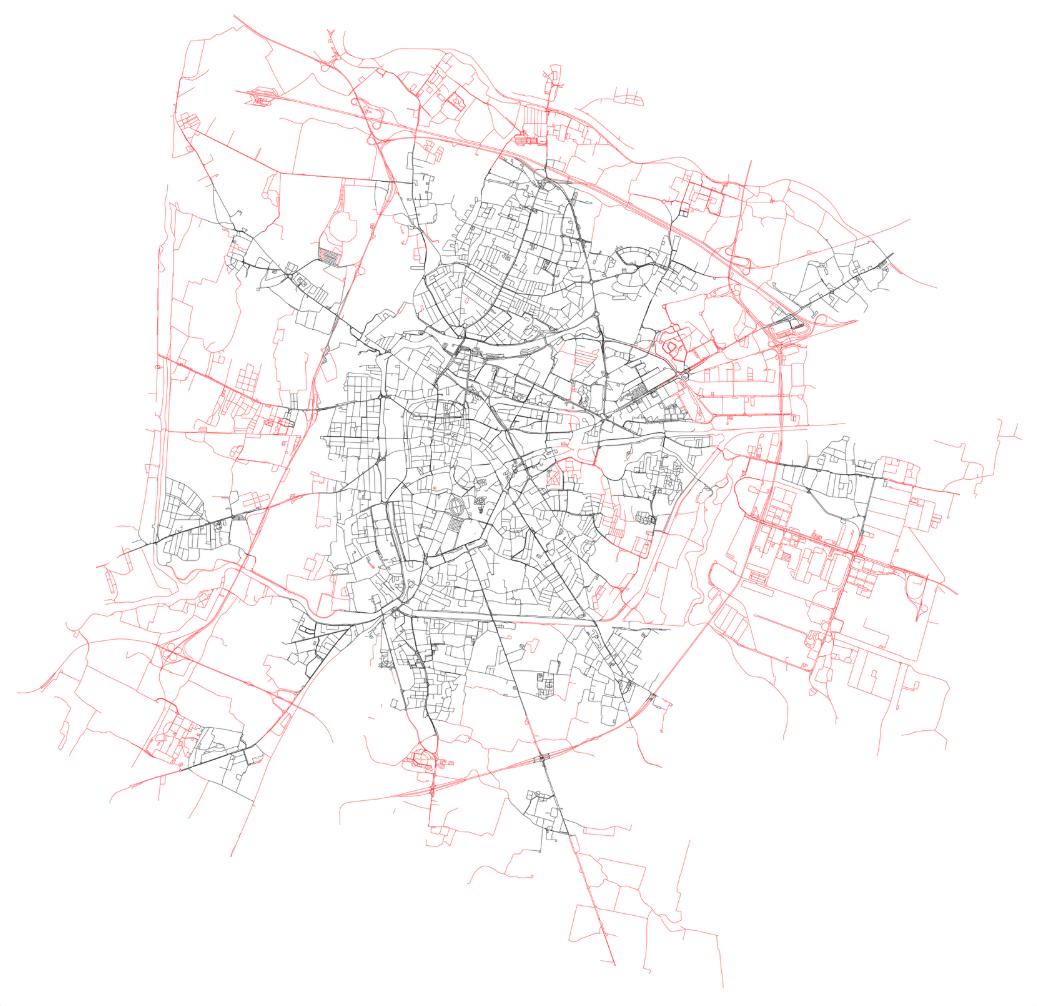
\includegraphics[width=\textwidth]{Padua_15MC.png}
    \caption{15-Minute City of Padua, Italy. Black edges represents the 15-Minute City.}
    \label{fig:padua_15MC}
\end{figure}

To measure the running time, we can run the algorithm repeatedly for 10000 iterations and take the average running time. The first 10 runs of the algorithm are excluded from the average to account for the warm-up time of the CPU. The average running time of the algorithm for the ``15-Minute City'' is \textbf{0.5} seconds.

\begin{table}[htbp]
    \begin{center}
        \caption{Padua t-Minute City}
        \label{tab:padua_tMC}
        \begin{tabular}{ccccc}
            \hline
            \textbf{$t$} & \textbf{Number of Nodes} & & \textbf{$t$} & \textbf{Number of Nodes} \\
            \hline
            \textbf{1} & 77 & & \textbf{16} & 8789 \\
            \textbf{2} & 310 & & \textbf{17} & 9123 \\
            \textbf{3} & 689 & & \textbf{18} & 9403 \\
            \textbf{4} & 1260 & & \textbf{19} & 9653 \\
            \textbf{5} & 1941 & & \textbf{20} & 9894 \\
            \textbf{6} & 2731 & & \textbf{21} & 10106 \\
            \textbf{7} & 3649 & & \textbf{22} & 10320 \\
            \textbf{8} & 4488 & & \textbf{23} & 10505 \\
            \textbf{9} & 5232 & & \textbf{24} & 10667 \\
            \textbf{10} & 5887 & & \textbf{25} & 10873 \\
            \textbf{11} & 6477 & & \textbf{26} & 11055 \\
            \textbf{12} & 7021 & & \textbf{27} & 11242 \\
            \textbf{13} & 7536 & & \textbf{28} & 11404 \\
            \textbf{14} & 8043 & & \textbf{29} & 11509 \\
            \textbf{15} & 8433 & & \textbf{30} & 11595 \\
            \hline
        \end{tabular}
    \end{center}
\end{table}

As discssed in Chapter \ref{intro}, ``15-Minute City'' is an urban city planning concept which we have seen many variations of in literature. This includes the study of 10, 20 and 30 minute cities. Therefore, we can run our algorithm multiple times to create a heatmap of the city of Padua for 1 to 30 minute cities. In summary, the number of nodes in the 1 to 30 minute cities can be seen in table \ref{tab:padua_tMC} and the heatmap of the $t$-Minute City of Padua can be seen in figure \ref{fig:padua_tMC}.

\textbf{Include average running time for each $t$}

\begin{figure}[htbp]
    \centering
    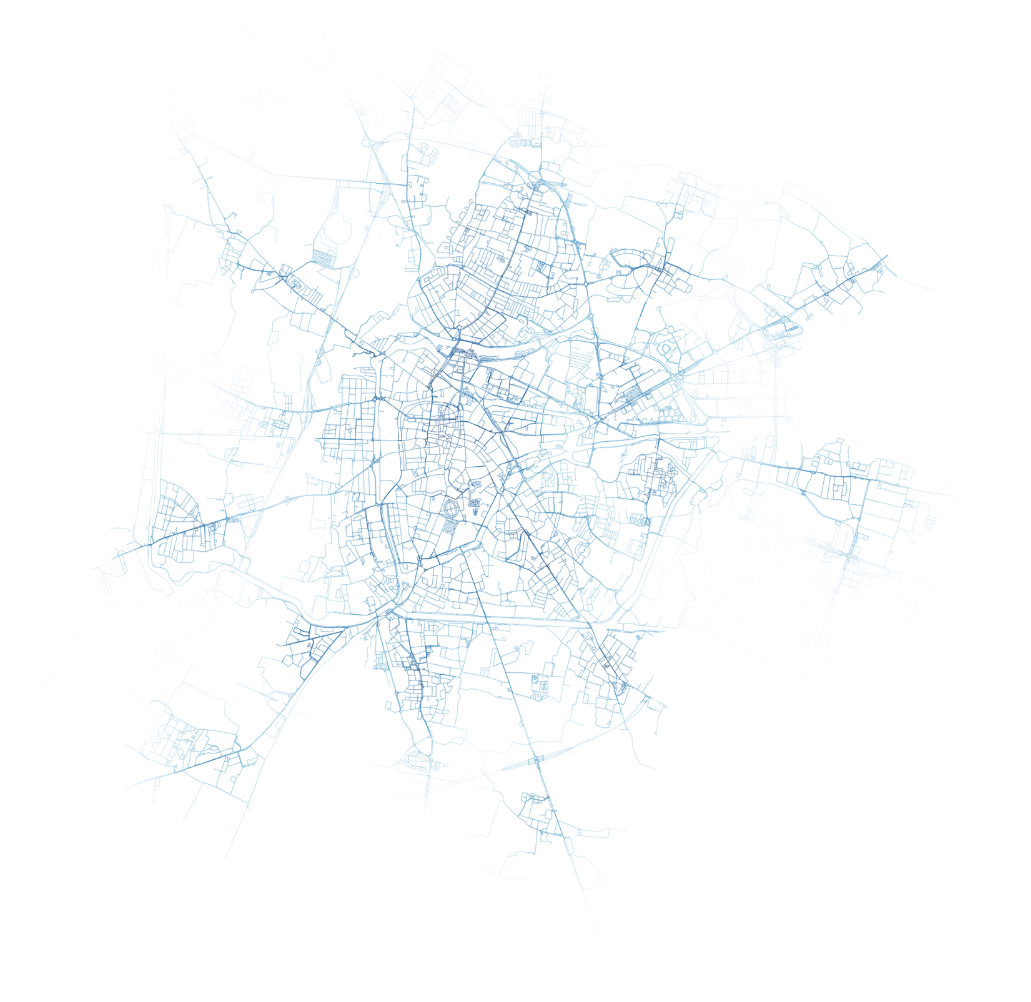
\includegraphics[width=\textwidth]{Padua_tMC.png}
    \caption{t-Minute City heatmap of Padua, Italy. Darker edges represnts a smaller $t$ value.}
    \label{fig:padua_tMC}
\end{figure}

\section{Adaption to existing papers}

In this section, we will apply our algorithm and compare with the results of the papers by Barbieri et al. in the cities of Rome, London and Paris \cite{barbieri_graph_2023}, Caselli et al. in the city of Parma, Italy \cite{caselli_exploring_2022} and Olivari et al. in the cities of Ferrara and Bologna of Italy \cite{olivari_are_2023}. We will discuss the usefulness of our algorithms, the similarities and differences between our results and theirs.

\subsection{Rome, London and Paris}

Noted by Barbieri et al. \cite{barbieri_graph_2023}, the planar graph of Rome, London and Paris were obtained from OpenStreetMap using the \verb|osmnx| library in Python. In the paper, the authors have defined 1.22 m/s as the average walking speed, which is the same as our experiment and slower than the average walking speed to be more inclusive to the population. The authors chose pharmacies, post office and supermarkets as the selected ammenities as the \say{three primary needs of food, health, and administration}. Bounding boxes of the 3 cities are also provided in the paper. However, the authors have not provided the \verb|network_type| parameter in the \verb|osmnx| library, which is important to obtain the correct map data. Furthermore, the authors have not mentioned any preprocessing steps to the map data, we also found that the bounding boxes provided in the paper are not accurate, as the bounding box of Paris did not provide the same area of the city as the figure shown in the paper.

Trying to recreate as close as possible to the map data used by the authors, figures \ref{fig:rome_15MC}, \ref{fig:london_15MC}, \ref{fig:paris_15MC} shows the comparison of the 15-Minute City of Rome, London and Paris, respectively, between our implementation and the results provided by Barbieri et al.

\textbf{Include figures}

\subsection{Parma, Italy} \label{parma}

Caselli et al. studied the 15-Minute City for the northern portion of the Cittadella district, Parma, Italy \cite{caselli_exploring_2022}. In the paper, the authors used a ArcGIS software with a GIS-model which improved and integrated a Territorial Information system. A walking speed of 3 km/h was used, which is equivalent to 0.83 m/s, the authors noted that this is due to a recommendation by the National Research Council (2000) \say{in urban areas with large numbers of older pedestrians}. A delay factor is also used in their model where the model adds 20 seconds to unsignalised crossings and 40 seconds to signalised crossings. This can be incorporated into our algorithm by adding the delay factor to the edge weights of the graph for crossings. The models used in this paper defined ``neighbour cores'' as \say{urban nodes well served by necessities shops and services, such as supermarkets, grocery
stores, bars, drugstores, and banks.} The ``15-Minute City'' is defined as the area where the ``neighbour cores'' are within 15 minutes of walking distance, the paper also separated the 16-Minute City into ``$0 - 5$ minutes'', ``$5 - 10$ minutes'' and ``$10 - 15$ minutes'' regions.

Since the authors did not include the coordinates of the ``neighbour cores'', nor the methodology used to obtain them. We will try to recreate the 15-Minute City of this area by simplily using the service types mentioned by the authors in our algorithm, along with the walking speed of 0.83 m/s. For the sake of simplisity, we will not include the delay factor in our model. Following our approach used in Section \ref{padua}, we will compute a heatamp of the 15-Minute City of the northern portion of the Cittadella district, Parma, Italy. The results of our implementation against Caselli et al. can be seen in figure \ref{fig:parma_tMC}.

\textbf{Include figures}

\subsection{Ferrara and Bologna, Italy}

In the paper by Olivari et al. \cite{olivari_are_2023}, the authors defined the ``Next Proximity Index'' and proposed the questions of whether the cities of Ferrara and Bologna, Italy are ``15-Minute''. Although the ``15-Minute City'' approach here is Grid Tessaletion based, the first ``Next Proximity Index'', NEXI-Minute for each service type is calculated by the time taken to reach to the clsoest service of the type, averaged from all nodes within the grid area. While the other two NEXI indices are built on top of the first index. Therefore, our algorithm can be used to aid with calculating the time taken to travel from each node to each service type. In this paper, the authors opted to use a walking speed of 5 km/h (1.39 m/s) without giving any specific reasons, and they have selected the following list of service types which are \say{mainly inspired by the Walk Score methodology} \cite{walkscore}.

\begin{enumerate}
    \item Commerce
    \item Retail
    \item Education
    \item Entertainment
    \item Grocery
    \item Healthcare
    \item Post/bank offices
    \item Public parks
    \item Restaurants
\end{enumerate}

Olivari et al. obtained the map data of Ferrara and Bologna from OpenStreetMap using the \verb|pandana| library in Python and with the \verb|network_type| as \verb|walk|. The authors provided a map visualising the averaged NEXI-Minute index over all service types of Ferrara. However, a specific OpenStreetMap tags for the service types were not provided. We will try to recreate the 15-Minute City of Ferrara and Bologna by using the service types mentioned by the authors in our algorithm, along with the walking speed of 1.39 m/s. The results of our implementation against Olivari et al. for the city of Ferrara can be seen in figure \ref{fig:ferrara_tMC} and figure \ref{fig:bologna_tMC} also shows our implementation of the city of Bologna.

\textbf{Include figures}

\section{Summary of complexity}

We have studied in Chapter \ref{proposed_solution} that the theorical complexity of our ``15-Minute City'' algorithm is

$$\mathcal{O}\left(p\cdot d^{1+\floor*{t/\epsilon}}\log d^{1+\floor*{t/\epsilon}}\right)\text{ and }O\left(p\cdot d^{1+\floor*{t/\epsilon}}\right)$$

In the table \ref{tab:complexity}, we have summarised the complexity of the algorithm for the ``15-Minute City'' of Padua, Rome, London, Paris, Parma, Ferrara and Bologna, along with the number of nodes and edges in each graph.

\begin{table}[htbp]
    \begin{center}
        \caption{Complexity in practice}
        \label{tab:complexity}
        \begin{tabular}{c|cccc}
            \hline
             & \textbf{|N|} & \textbf{|E|} & \textbf{Complexity} \\
            \hline
            \textbf{Padua} & 12535 & 18706 & 3 \\
            \textbf{Rome} & 12535 & 18706 & 3 \\
            \textbf{London} & 12535 & 18706 & 3 \\
            \textbf{Paris} & 12535 & 18706 & 3 \\
            \textbf{Parma} & 12535 & 18706 & 3 \\
            \textbf{Ferrara} & 12535 & 18706 & 3 \\
            \textbf{Bologna} & 12535 & 18706 & 3 \\
            \hline
        \end{tabular}
    \end{center}
\end{table}

\textbf{Also measure different $t$?}